\documentclass[11pt, oneside]{article}   	% use "amsart" instead of "article" for AMSLaTeX format
\usepackage{geometry}                		% See geometry.pdf to learn the layout options. There are lots.
\geometry{letterpaper}                   		% ... or a4paper or a5paper or ... 
%\geometry{landscape}                		% Activate for for rotated page geometry
%\usepackage[parfill]{parskip}    		% Activate to begin paragraphs with an empty line rather than an indent
\usepackage{graphicx}				% Use pdf, png, jpg, or eps� with pdflatex; use eps in DVI mode
								% TeX will automatically convert eps --> pdf in pdflatex		
\usepackage{amssymb}
\usepackage{amsmath}
\usepackage{parskip}
\usepackage{color}
\usepackage{hyperref}

\title{Fourier Series:  cofactors}
%\author{The Author}
%\section{}
%\subsection*{}
\date{}							% Activate to display a given date or no date

\graphicspath{{/Users/telliott_admin/Dropbox/Tex/png/}}
% \begin{center} 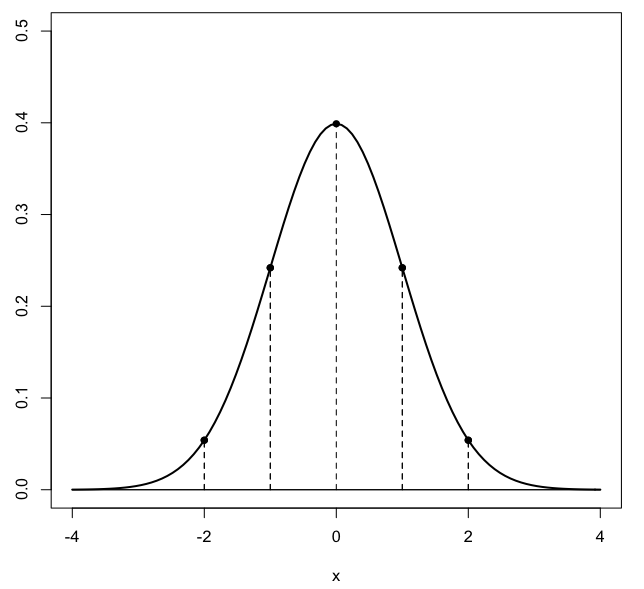
\includegraphics [scale=0.4] {gauss3.png} \end{center}
\begin{document}
\maketitle
\Large
You have some periodic function and you've decided to approximate it using a Fourier series.  You write
\[ f(x) = \sum_{n=0}^{\infty} A_n \cos\frac{n\pi x}{L} + \sum_{n=1}^{\infty} B_n \sin\frac{n\pi x}{L} \]
How to determine the cofactors? Multiply every term by $\cos m\pi x/L, m = 0$ and then integrate between $-L \rightarrow L$.
\[ \int_{-L}^L f(x) \ dx = \dots \]
In the series on the right-hand side, every term except the first one goes away.  What's left is
\[ \int_{-L}^L f(x) \ dx = A_0 \cos 0 = A_0 \]


\end{document}  